\documentclass[]{tufte-book}

% ams
\usepackage{amssymb,amsmath}

\usepackage{ifxetex,ifluatex}
\usepackage{fixltx2e} % provides \textsubscript
\ifnum 0\ifxetex 1\fi\ifluatex 1\fi=0 % if pdftex
  \usepackage[T1]{fontenc}
  \usepackage[utf8]{inputenc}
\else % if luatex or xelatex
  \makeatletter
  \@ifpackageloaded{fontspec}{}{\usepackage{fontspec}}
  \makeatother
  \defaultfontfeatures{Ligatures=TeX,Scale=MatchLowercase}
  \makeatletter
  \@ifpackageloaded{soul}{
     \renewcommand\allcapsspacing[1]{{\addfontfeature{LetterSpace=15}#1}}
     \renewcommand\smallcapsspacing[1]{{\addfontfeature{LetterSpace=10}#1}}
   }{}
  \makeatother
\fi

% graphix
\usepackage{graphicx}
\setkeys{Gin}{width=\linewidth,totalheight=\textheight,keepaspectratio}

% booktabs
\usepackage{booktabs}

% url
\usepackage{url}

% hyperref
\usepackage{hyperref}

% units.
\usepackage{units}


\setcounter{secnumdepth}{-1}

% citations
\usepackage{natbib}
\bibliographystyle{plainnat}

% pandoc syntax highlighting
\usepackage{color}
\usepackage{fancyvrb}
\newcommand{\VerbBar}{|}
\newcommand{\VERB}{\Verb[commandchars=\\\{\}]}
\DefineVerbatimEnvironment{Highlighting}{Verbatim}{commandchars=\\\{\}}
% Add ',fontsize=\small' for more characters per line
\newenvironment{Shaded}{}{}
\newcommand{\KeywordTok}[1]{\textcolor[rgb]{0.00,0.44,0.13}{\textbf{#1}}}
\newcommand{\DataTypeTok}[1]{\textcolor[rgb]{0.56,0.13,0.00}{#1}}
\newcommand{\DecValTok}[1]{\textcolor[rgb]{0.25,0.63,0.44}{#1}}
\newcommand{\BaseNTok}[1]{\textcolor[rgb]{0.25,0.63,0.44}{#1}}
\newcommand{\FloatTok}[1]{\textcolor[rgb]{0.25,0.63,0.44}{#1}}
\newcommand{\ConstantTok}[1]{\textcolor[rgb]{0.53,0.00,0.00}{#1}}
\newcommand{\CharTok}[1]{\textcolor[rgb]{0.25,0.44,0.63}{#1}}
\newcommand{\SpecialCharTok}[1]{\textcolor[rgb]{0.25,0.44,0.63}{#1}}
\newcommand{\StringTok}[1]{\textcolor[rgb]{0.25,0.44,0.63}{#1}}
\newcommand{\VerbatimStringTok}[1]{\textcolor[rgb]{0.25,0.44,0.63}{#1}}
\newcommand{\SpecialStringTok}[1]{\textcolor[rgb]{0.73,0.40,0.53}{#1}}
\newcommand{\ImportTok}[1]{#1}
\newcommand{\CommentTok}[1]{\textcolor[rgb]{0.38,0.63,0.69}{\textit{#1}}}
\newcommand{\DocumentationTok}[1]{\textcolor[rgb]{0.73,0.13,0.13}{\textit{#1}}}
\newcommand{\AnnotationTok}[1]{\textcolor[rgb]{0.38,0.63,0.69}{\textbf{\textit{#1}}}}
\newcommand{\CommentVarTok}[1]{\textcolor[rgb]{0.38,0.63,0.69}{\textbf{\textit{#1}}}}
\newcommand{\OtherTok}[1]{\textcolor[rgb]{0.00,0.44,0.13}{#1}}
\newcommand{\FunctionTok}[1]{\textcolor[rgb]{0.02,0.16,0.49}{#1}}
\newcommand{\VariableTok}[1]{\textcolor[rgb]{0.10,0.09,0.49}{#1}}
\newcommand{\ControlFlowTok}[1]{\textcolor[rgb]{0.00,0.44,0.13}{\textbf{#1}}}
\newcommand{\OperatorTok}[1]{\textcolor[rgb]{0.40,0.40,0.40}{#1}}
\newcommand{\BuiltInTok}[1]{#1}
\newcommand{\ExtensionTok}[1]{#1}
\newcommand{\PreprocessorTok}[1]{\textcolor[rgb]{0.74,0.48,0.00}{#1}}
\newcommand{\AttributeTok}[1]{\textcolor[rgb]{0.49,0.56,0.16}{#1}}
\newcommand{\RegionMarkerTok}[1]{#1}
\newcommand{\InformationTok}[1]{\textcolor[rgb]{0.38,0.63,0.69}{\textbf{\textit{#1}}}}
\newcommand{\WarningTok}[1]{\textcolor[rgb]{0.38,0.63,0.69}{\textbf{\textit{#1}}}}
\newcommand{\AlertTok}[1]{\textcolor[rgb]{1.00,0.00,0.00}{\textbf{#1}}}
\newcommand{\ErrorTok}[1]{\textcolor[rgb]{1.00,0.00,0.00}{\textbf{#1}}}
\newcommand{\NormalTok}[1]{#1}

% longtable

% multiplecol
\usepackage{multicol}

% strikeout
\usepackage[normalem]{ulem}

% morefloats
\usepackage{morefloats}


% tightlist macro required by pandoc >= 1.14
\providecommand{\tightlist}{%
  \setlength{\itemsep}{0pt}\setlength{\parskip}{0pt}}

% title / author / date
\title{Introduction to R and R Studio}
\date{January 01 2018}


\begin{document}

\maketitle




\chapter{Overview of R and RStudio}\label{overview-of-r-and-rstudio}

From the outset, we need to recognize that there are lots of valuable
standalone programs for evolutionary genetic analysis, many of which
operate on Windows, Mac and Linux platforms and do so in a user-friendly
fashion. However, there is one serious downside to exclusive dependence
on such packages - many of them require specialized data formats, and
outputs from one such program are often not readily input into another.

R \citep{RHome}, on the other hand, has a couple of advantages:

\section{It is a data oriented programming
language,}\label{it-is-a-data-oriented-programming-language}

so virtually any data can be input in some form or another. For example,
one can directly read data from
\href{http://alfred.med.yale.edu}{ALFRED},
\href{http://www.datadryad.org}{Dryad} and other such data bases, and
with some manipulation (a. k. a. munging) get them into a format that
can be used for a wide variety of applications.

\section{R is vector-based}\label{r-is-vector-based}

For those who remember the days of having to wrestle with subscript
indices in languages like FORTRAN and BASIC, R is a delight. For
example, suppose you wish to create a vector of integers from 1:100. It
is as easy as

\begin{Shaded}
\begin{Highlighting}[]
\NormalTok{x=}\KeywordTok{c}\NormalTok{(}\DecValTok{1}\OperatorTok{:}\DecValTok{100}\NormalTok{)}
\NormalTok{x}
\end{Highlighting}
\end{Shaded}

\begin{verbatim}
##   [1]   1   2   3   4   5   6   7   8   9  10
##  [11]  11  12  13  14  15  16  17  18  19  20
##  [21]  21  22  23  24  25  26  27  28  29  30
##  [31]  31  32  33  34  35  36  37  38  39  40
##  [41]  41  42  43  44  45  46  47  48  49  50
##  [51]  51  52  53  54  55  56  57  58  59  60
##  [61]  61  62  63  64  65  66  67  68  69  70
##  [71]  71  72  73  74  75  76  77  78  79  80
##  [81]  81  82  83  84  85  86  87  88  89  90
##  [91]  91  92  93  94  95  96  97  98  99 100
\end{verbatim}

No need to set dimenstions or any of that stuff. And we can then do
simple manipulations on those objects, such as

\begin{Shaded}
\begin{Highlighting}[]
\NormalTok{x}\OperatorTok{*}\DecValTok{2}
\end{Highlighting}
\end{Shaded}

\begin{verbatim}
##   [1]   2   4   6   8  10  12  14  16  18  20
##  [11]  22  24  26  28  30  32  34  36  38  40
##  [21]  42  44  46  48  50  52  54  56  58  60
##  [31]  62  64  66  68  70  72  74  76  78  80
##  [41]  82  84  86  88  90  92  94  96  98 100
##  [51] 102 104 106 108 110 112 114 116 118 120
##  [61] 122 124 126 128 130 132 134 136 138 140
##  [71] 142 144 146 148 150 152 154 156 158 160
##  [81] 162 164 166 168 170 172 174 176 178 180
##  [91] 182 184 186 188 190 192 194 196 198 200
\end{verbatim}

And every element is multiplied by 2.

\section{And we can do plots.}\label{and-we-can-do-plots.}

Working with our same vector, we can easily get a simple working plot by

\begin{Shaded}
\begin{Highlighting}[]
\KeywordTok{plot}\NormalTok{(x)}
\end{Highlighting}
\end{Shaded}

\begin{marginfigure}
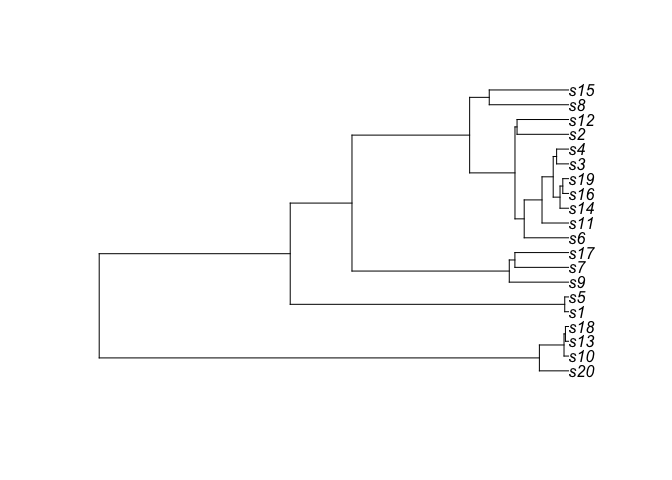
\includegraphics{NewIntroR_files/figure-latex/unnamed-chunk-3-1} \caption[This plot, as well as the following, are done in "base graphics"]{This plot, as well as the following, are done in "base graphics".  We will introduce more sophisticated graphics in the chapter on the "tidyverse"}\label{fig:unnamed-chunk-3}
\end{marginfigure}

And we get the plot seen to the right.

\section{R is imminently extensible}\label{r-is-imminently-extensible}

with both built-in functions that carry out complex tasks based on
simple commands, as well as add on packages that provide additional
capabilities for specialized tasks. For example, suppose we want to
generate a bunch of random binomial variants, akin to doing 100
experiments of flipping a coin 100 times qne plotting how many heads we
get. We can write

\begin{Shaded}
\begin{Highlighting}[]
\NormalTok{h <-}\KeywordTok{rbinom}\NormalTok{(}\DecValTok{100}\NormalTok{,}\DecValTok{100}\NormalTok{,.}\DecValTok{5}\NormalTok{)}
\KeywordTok{hist}\NormalTok{(h)}
\end{Highlighting}
\end{Shaded}

\begin{marginfigure}
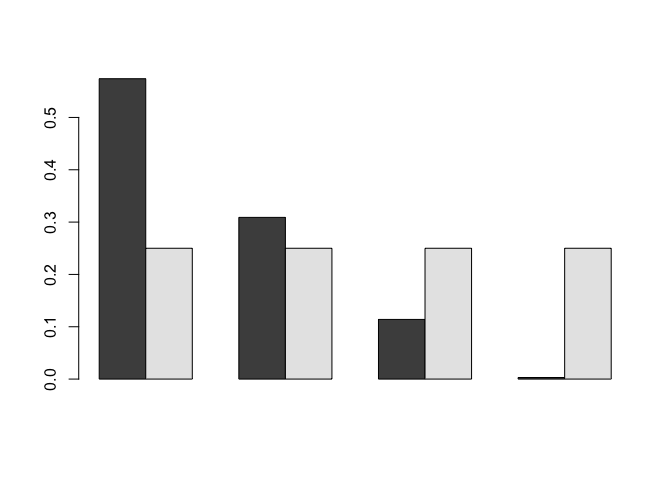
\includegraphics{NewIntroR_files/figure-latex/unnamed-chunk-4-1} \end{marginfigure}

\section{And then there are
packages.}\label{and-then-there-are-packages.}

R is open source, so there are legions of skilled programmers
specifically developing add-on packages that can be installed and
provide additional functionality. We will use a lot of these packages,
including

\begin{quote}
\begin{itemize}
\tightlist
\item
  ape \citep{Paradis2004} and pegas \citep{Paradis2010} - provide
  essential functions for population genetic analysis and tree
  manipulation
\item
  phyclust \citep{Phyclust} - an independently developed package that
  has the interesting ability to run some otherwise command-line
  stand-alone programs (ms \citep{ms}, seq-gen) directly within R
\item
  rehh \citep{rehh} - Brings the world of Pardis Sabeti and extended
  haploytpe analaysis to R. Data munging is challenging, but once done,
  it is rewarding.
\end{itemize}
\end{quote}

\chapter{RStudio}\label{rstudio}

By itself, R can be intimidating. In particular, it is a ``command
line'' program, meaning that once a command is entered, it is executed,
something that is not necessarily desirable when performing complex
tasks. The program becomes much more functional if multiple lines of
code can be entered simultaneously, and importantly \emph{the code can
be annotated such that a reader can understand what's being done}.

RStudio is an ``Integrated Development Environment'', or IDE, that
greatly facilitates working with R, and quite importantly documenting
that work.

\section{Installation is easy}\label{installation-is-easy}

Go to RStudio.org, look for the download program for your
platform(Windows, Mac or whatver) and download it. Windows will probably
have to be unzipped and executed; Mac will come as a DMG file that has
to be installed. But be assured that in just a few minutes (I did it
while wating to board a plane) you will have the system up and running.

When you open RStudio, you are presented with four panes.

1.The upper left is where you do most of the work, it is here you can
type sets of commpands, run them and see what happens, 2. You can enter
single commands in the lower left that will execute when you hit return,
however the more valuable role of that panel is to display numerical
results that arise for the command blocks you run in the upper left
pane. 3. The upper right pane I think of a s a bookeeping area. It
provides a list of all of the objects that are available in memory (and
thus can be used in the currnet session). It gives the object name, as
well as the nature of the object (vector, matrix, list, data frame, and
many others.) 4. The lower right is where the graphs appear, and this is
the fun stuff. R is exceptionally good at providing visualization of
data in ways that can be readily interpreted; much of what we do will
focus on interpretation of this output.

\section{\texorpdfstring{Creating a ``Markdown'' file for Program
Execution}{Creating a Markdown file for Program Execution}}\label{creating-a-markdown-file-for-program-execution}

This is the coolest feature of R studio. The best place to start is with
the video below, in which Roger Peng of Johns Hopkins runs you through
the basics of what we'll be doing.

Suppose I've written a file that includes some text (such as this) as
well as ``chunks'' of code that can be executed. The code is sparated by
the following delimiters:

```\{r\}\\
\#Code goes here\\
```

When the HTML rendered, or knitted, you will see the actual coded in a
shaded box, followed by the result of that code's execution in an
unshaded one. Everything outside the chunk will be treated as regular
text and formatted accordingly.

\section{Publishing as HTML}\label{publishing-as-html}

So up to this point, we have completed a narrative describing some
basics of R and RStudio, and we have embedded a few chunks of code to
illustrate some points. What we would now like to do would be to publish
our writing in a format that is broadly accessible to others. To do so,
RStudio has the package ``knitr'' built in, which will render a markdown
document (such as this) in standard html, accessible from any browser.
To do so is simple - either click the ``Knit HTML'' button at the top of
the window, or press Shift-Command-H. If you haven't done so already,
you will be prompted for a file name for saving the R Markdown file (it
will have the suffix .Rmd added). Two additional files will then be
generated - a markdown file, which can be accessed by other programs for
format tweaking and so forth, but most importantly, an html file that
can then be opened in any browser.

\chapter{Getting Help}\label{getting-help}

The philosophy of this project is that the reader should learn by doing.
Thus, we won't spend a whole lot of time dealing with the minutiae of
the R programming language; rather we will introduce particular
functions and concepts in the context of actual problems. However, there
are several places the user can turn for quick assistance:

\section{R Help pages}\label{r-help-pages}

Simply entering ?function on the command line (in the lower left pane)
will bring up the standard help page for that function. While these
pages are sometimes cryptic, they should include

\begin{quote}
\begin{itemize}
\tightlist
\item
  A brief description of what the function does
\item
  A description of its syntax
\item
  The nature of the arguments that the function uses
\item
  The value that is returned
\item
  (usually) a few examples of its uses
\end{itemize}
\end{quote}

In the case of packages, the easiest way to get documentation in RStudio
is to select the ``Package'' tab in the lower right pane of the RStudio
display and click on the package of interest. That will bring up a page
with links to information on that package, and most importantly to the
help files for all of the functions contained within it.

\section{Markdown syntax}\label{markdown-syntax}

Markdown is probably the easiest way to embed basic formatting
information into a document, in such a way that is can be rendered into
a publishable format. A good general introduction to it can be found
\href{http://net.tutsplus.com/tutorials/tools-and-tips/markdown-the-ins-and-outs/}{here};
a description of its use in Rstudio can be found
\href{http://www.rstudio.com/ide/docs/authoring/using_markdown}{here}.

\chapter{Summary}\label{summary}

So at this point, where are we?

\begin{enumerate}
\def\labelenumi{\arabic{enumi}.}
\tightlist
\item
  We gave R and R Studio up and running
\item
  We have performed some basic data retrieval and made a bar plot
\item
  We have rendered our narrative and code into HTML so that it can be
  accessed on the web.
\end{enumerate}

But, you ask, what good is all of this? How do we address real questions
with real data? To get there, we need to spend a bit of time looking at
at least a few of R's capabilities with respect to data manipulation.

\renewcommand\bibname{References}
\bibliography{../TPG.bib}



\end{document}
